\chapter{Protein-GAG binding site prediction via electrostatic potential analysis}

In this chapter we present a simple and yet efficient method for predicting
where on a protein a GAG would most likely bind, suggesting which amino acid
residues are likely to be involved in the interaction and which are not. The
method is based on numerical simulation of the electrostatic (i.e.\ Coulomb)
potential of the protein in water solution, and manual evaluation of the
topology of the Coulomb potential in space. Subsequently, we apply that method
to IL-10 and report our findings.

\section{Motivation}

Classical molecular docking approaches are used for creating binding predictions
for a given receptor-ligand system. Primarily, the correctness of a prediction
depends on the quality of the underlying physical or phenomenological model, and
whether the system under investigation is within the scope of validity of the
model. Since most molecular docking methods are trained for analyzing a limited
Cartesian volume in a \textit{local} search, application to larger search spaces
such as in \textit{global} docking dramatically lowers the confidence in the
resulting prediction. Therefore, common molecular docking methods should be
applied locally, and hence require \textit{a priori} knowledge about where on
the receptor the ligand most likely binds. The decision where to center the
local search on should be based on reliable data, otherwise the docking study
might be pointless. In the best case, knowledge about the binding site (the
region on the receptor that the ligand binds to) comes from experimental data,
e.g.\ from mutagenesis or NMR studies. However, in many cases no such
experimental data is available, as is unfortunately true for the IL-10-GAG
system. In such situations, it makes sense to consider \textit{in silico}
methods for binding site prediction.

With respect to protein-GAG systems, there is only few published work on this
topic. In \cite{hp_binding_sites_mulloy_2006}, Forster and Mulloy used AutoDock
version 2.4 \cite{autodock24} for globally docking rigid heparin molecules to
antithrombin and FGF2, and found that their docking procedure gave good
agreement with the corresponding crystal structures regarding the overall
position of the heparin binding sites. The authors state that the method may be
used as \enquote{hypothesis generation tool} rather than for providing
\enquote{details of interactions between specific atoms}. In another work
\cite{gandhi_bmp_heparin_binding_sites_2012}, the authors used PatchDock
\cite{patchdock_2002} for globally docking rigid heparin oligosaccharides to
BMP-2 and BMP-14 and state that \enquote{while there has been no validation of
the accuracy of the PatchDock scoring function for heparin interactions, these
docking results suggest the presence of two GAG binding sites in BMP-2}. In
\cite{rogers_gag_prot_prot_2011}, the authors used a mixture of two docking
softwares for rigid-body docking of GAG structures \enquote{to the entire
molecular surface of the protein to locate the most favorable binding sites}.
Also in \cite{bitomsky_gag_docking_1999}, the authors report success in
predicting heparin binding sites on proteins using various docking methods.

The above-cited studies do by no means provide a complete picture, but obviously
some of the established docking methods seem to be able to reflect certain
properties of protein-GAG systems. This is remarkable since none of these
docking methods has been specifically optimized for GAG ligands, let alone for
global docking, and strictly spoken, when applied to protein-GAG systems, these
docking methods are applied outside their scope of validity. We postulate that
the reason for the surprising success in named studies is that protein-GAG
complexes are strongly driven by Coulomb interaction and that mentioned docking
methods incorporate Coulomb interaction with a significant weight in their
scoring functions.

In fact, heparin has the highest negative charge density among biological
macromolecules \cite{capila_linhardt_hep_prot_2002}. Standard literature on
protein-GAG systems such as
\cite{essentials_glycobiology_gags_2009,gandhi_structure_2008} stresses the
role of charge-charge interaction in protein-GAG systems in general. Many
publications focusing on individual protein-GAG systems identify charge
complementary as one of the driving mechanisms of the interaction between GAG
and protein
\cite{gandhi_bmp_heparin_binding_sites_2012,faham_heparin_1996,%
pichert_characterization_2012,rogers_gag_prot_prot_2011}.

We can conclude that the importance of Coulomb interaction is a distinctive
feature of protein-GAG systems. Notably, compared to other molecular interaction
types, the Coulomb interaction is a long range interaction and therefore
dominates all other contributions for larger distances. As of these
considerations, it seems to be reasonable to perform protein-GAG binding site
prediction purely based on the strength and topology (i.e.\ the
shape/distribution) of the electrostatic potential in the volume surrounding the
protein.

For a set of reference systems, we have investigated the relation between the
strength and topology of Coulomb potential and the actual experimentally
determined GAG binding site in order to determine whether the electrostatic
properties alone can assist in predicting a receptor GAG binding site. The
result of this study, be it positive or negative, in any case further enlightens
the role of Coulomb interaction in protein-GAG systems.


\section{Method}

\subsection{Coulomb potential simulation}

For a given protein, we calculated its electrostatic potential with a
finite-difference numerical solver applied to the linearized Poisson-Boltzmann
(PB) equation. The PB equation is widely used for implementing a class of
implicit solvent models to describe solvent-mediated electrostatic interactions.
These models have been demonstrated to be reliable in reproducing the energetics
when compared with explicit solvent molecular dynamics simulations and
experimental measurements for a wide range of systems \cite{honig_estatic_1995}.
In the PB model we have applied, the solute (protein) is described by an
atomic-detail representation, while the solvent molecules are treated as a
continuum. The solute is modeled as a dielectric body whose shape is defined by
atomic coordinates and atomic radii. A set of point charges at the atomic
centers produces an electrostatic field in the solute region as well in the
solvent region. The overall electrostatic field is the sum of the Coulombic
field of the solute and the corresponding reaction field of the polarizable
solvent.

We used the PBSA program shipped with AmberTools 13 \cite{case_amber_12} with
default parameters and a finite element grid spacing of \SI{1}{\angstrom} for
calculating the overall electrostatic potential of any given protein in water.
The atomic radii and point charges of the protein were parameterized according
to the FF99SB force field \cite{case_amber_12}. After patching PBSA (and
contributing those patches back to the AmberTools project), we were able to
extract the Coulomb data from PBSA in units of
\si{\kilo\calory\per\mole\per\elementarycharge} and in a file format readable by
the visualization software VMD \cite{vmd_1996}.

\subsection{Coulomb potential evaluation}

Many authors discussing the properties of a certain GAG receptor protein depict
the electrostatic potential of the protein mapped onto its molecular surface, as
done in \cite{rogers_gag_prot_prot_2011,%
Gandhi01102009,sapay_hs_growthfactors_2011,%
gandhi_bmp_heparin_binding_sites_2012,sost_heparin_2009,%
catK_cs4_crystal_structure_2008,hydrolase_gags_2011,gandhi_structure_2008,%
imberty_gag_prot_carbres_2007,gags_as_polyelectrolytes_2010}. Most of these
works lack clear conclusions from this kind of analysis, which in our opinion is
the result of two conceptual flaws of the approach. First of all, by only
looking at the surface one ignores the properties of the potential in the volume
surrounding the protein, i.e.\ one misses to analyze how a GAG in vicinity of a
protein may be guided by a certain topology of the potential in space. Secondly,
an unfortunately often overseen disadvantage of the surface-mapping approach is
that the PB approximation of the electrostatic potential is
\text{most} error-prone near the dielectric boundary, i.e.\ right on the
molecular surface. In \cite{estatic_proteins_warshel_2006}, Warshel et al.\
write that \enquote{the problem is not the well-known bulk contribution from the
surroundings [\dots], but the polarization at the microscopic boundaries of the
simulation spheres}.

The data we obtain from PBSA are the values of the electrostatic potential on
the grid centers of a three-dimensional grid, spanning a volume of a certain
size including the protein as well as its surroundings. In contrast to what is
usually done, we decided to analyze the properties of the electrostatic
potential within the entire protein-surrounding volume, \textit{i)} for working
around the uncertainty of the data near the boundary, and \textit{ii)} for
looking at the complete picture.

We therefore analyzed the topology and strength of the potential with an
isosurface representation while varying the isosurface value. This procedure,
which will become more clear in \cref{bspred:appl_discussion} below, allows for
understanding the distribution of the potential in space as well as how strongly
it would affect a ligand. A characteristic isovalue was determined individually
for each protein for the case where only a small part of the isosurface is
protruding into space further than the molecular surface of the receptor. This
characteristic isovalue may provide an idea about the strength of the
electrostatic interaction between ligand and receptor in the bound state. The
isosurface visualization was performed using VMD \cite{vmd_1996}.

\section{Application to reference systems}
\label{bspred:application}

We have analyzed the electrostatic potential of the following well-understood
and experimentally characterized protein-GAG systems: basic fibroblast growth
factor (FGF2) in complex with a heparin (HP) tetrasaccharide, PDB ID 1BFB,
\SI{1.9}{\angstrom} resolution; the CD44 hyaluronic acid binding domain in
complex with a hyaluronan heptasaccharide (HA), PDB ID 2JCQ,
\SI{1.3}{\angstrom}; and stromal cell-derived factor-1 (SDF-1) in complex with a
HP disaccharide, PDB ID 2NWG, \SI{2.1}{\angstrom}.

Furthermore, we have applied the electrostatic potential analysis to Sclerostin
(SOST), whose interaction with heparin has recently been investigated via NMR
\cite{sost_heparin_2009}.

\subsection{Results and discussion}
\label{bspred:appl_discussion}

\begin{figure}
\centering
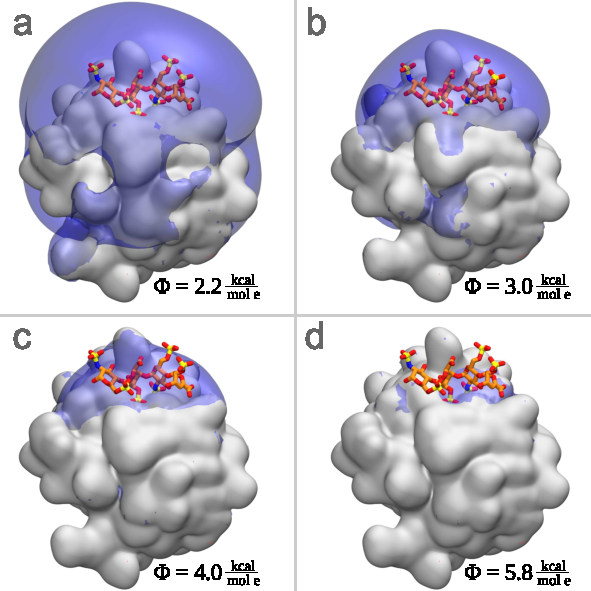
\includegraphics[width=0.9\textwidth]{gfx/bspred/fgf2_coulomb_isosurfaces_different_values_03_ds.pdf}
\caption[]{
Isosurface representation of FGF2's Coulomb potential (blue), shown for four
different isovalues isovalues $\Phi$, in increasing order. The molecular surface
of FGF2 is shown in gray, its heparin ligand pose as determined experimentally
is shown as sticks with carbon atoms in orange (structure taken from PDB ID
1BFB).}
\label{fig:bspred:fgf2_multi_iso}
\end{figure}

\Cref{fig:bspred:fgf2_multi_iso} depicts the process of visualizing the
electrostatic potential of FGF2 with an isosurface representation and varying
isovalue. The four isovalues shown are positive ones, and the isosurfaces
therefore represent \textit{attraction} for GAGs. Isosurfaces for isovalues of
comparable absolute value and opposite sign are \enquote{within} the molecular
surface, i.e.\ electrostatic GAG \textit{repulsion} is negligible in case of
FGF2.

\Cref{fig:bspred:fgf2_multi_iso}a shows the isosurface corresponding to the
smallest of the four isovalues with
\SI{2.2}{\kilo\calory\per\mole\per\elementarycharge}. This is still a strong
potential, yielding significant potential energies for charged ligand molecules:
\SI{2.2}{\kilo\calory\per\mole} is almost four times larger than the thermal
energy at \SI{300}{\kelvin}. From this representation we learn that FGF2 is
highly polar on a global scale: in the depicted top direction, the isosurface
protrudes into space far beyond the molecular surface, whereas it does not
surpass the molecular surface at the bottom. We conclude that FGF2 may interact
with GAGs over large distances (several times larger than what can be
considererd a molecular contact), and with a clear preference towards one side
of the protein (the top in \Cref{fig:bspred:fgf2_multi_iso}). Furthermore, we
observe that the experimentally determined natural heparin ligand pose is bound
to exactly that side of FGF2.

\Cref{fig:bspred:fgf2_multi_iso}b and c visualize the process of increasing
the isovalue while observing the response of the isosurface. This process serves
two purposes. Firstly, isosurface shape changes with increasing isovalue provide
insight about the direction into which a negatively charged molecule would be
\textit{guided} by the electrostatic potential once caught (the gradient of the
potential). Secondly, it allows for further narrowing down those regions in
space near the molecular surface of FGF2 where electrostatic attraction is
strongest, because the surface protrudes less and less into space with
increasing isovalue. Regarding directionality, the isosurface clearly contracts
itself towards a certain region on FGF2's surface, considering panels a, b, and
c of \Cref{fig:bspred:fgf2_multi_iso}. It is that region where we also find the
experimentally determined ligand pose. In panel c weobserve that there is only a
small region in space outside of FGF2 where the electrostatic potential is as
large as \SI{4.0}{\kilo\calory\per\mole\per\elementarycharge}, which is about
seven times stronger than the thermal energy at room temperature, considering
a single test charge.


per elementary charge,
which is about



changes in the shape of the isosurface shown For the isovalue shown in \Cref{fig:bspred:fgf2_multi_iso}c, we
observe that



identification of those regions in
space and therefor e



in \Cref{fig:bspred:fgf2_multi_iso} we observe that

is able to \enquote{catch} GAGs via electrostatic attaction from quite a
distance, with a clear preference--- with one


the top direction, whereas



visualization


Regarding the SDF-1-HP complex, our electrostatic potential evaluation procedure
unambiguously identifies the GAG binding site as determined experimentally. With
$8.5\,\mathrm{kcal\,mol^{-1}\,e^{-1}}$, the isovalue chosen is the largest among
the TDS complexes, indicating that SDF-1 has the strongest electrostatic
attraction to its ligand. In case of FGF2-HP (\cref{fig:bspred:various_estatic}), the
binding site is also unambiguously defined by the electrostatic potential.







\cref{fig:bspred:sdf1_estatic} shows an isosurface of
the Coulomb potential of SDF-1.
\cref{fig:bspred:various_estatic} shows analogous isosurface representations of
the electrostatic potential for the other TDS complexes.










TODO: argue, why application of complex docking methods only allowed us to
speculate why they are sometimes succcessfull (see motivation part), but now,
in a controlled environment with a very simple model (only coulomb), we can
directly conclude that coulomb interaction IS the dominating interaction that
alone determines binding site for many systems.


Discuss: The most important aspect to discuss regarding a method for predicting
certain behavior is the certainty of the prediction. we can conclude that this
method is very well able to make valid predictions regarding protein-GAG binding
regions. Compared to docking methods, this method is significantly less complex:
it is a bare-bones method, incorporating a quite simple physical model, whereas
docking methods usually apply a combination of physical as well as
phenomenological model. The certainty of a docking prediction is difficult to
assess if the docking method is applied outside its scope of validity, i.e.\ to
different systems and search space sizes than it has been developed for.
Strictly spoken, the certainty is not assessable, neither quantitatively, nor
qualitatively. The reason for this is the large complexity of a docking method,
as of which we can not systematically describe how the method should behave, if
we leave the scope of validity.

compared to simple electrostatic potential evaluation.

The prediction method we have presented here, however, seems to provide a good
estimate about the certainty of its prediction. We see that the data about CD44
is inconclusive, at the same time the data regarding FGF2 and SDF-2 as well as
SOST provides strong evidence that GAGs bind where predicted, especially regarding
the large characteristic electrostatic potential isovalues in proximity of the
molecular surface. This is a huge advantage.



Discuss FGF2, SDF1, and CD44!

Refer to \hl{The result of this study, be it positive or negative, in any case
further enlightens the role of Coulomb interaction in protein-GAG systems.}

\section{Application to IL-10}

Regarding IL-10, the shape of the potential in space provides strong evidence
that if GAGs bind to it, then most likely in a well-defined region. What makes
this prediction less certain as e.g.\ in case of SDF-1 and FGF2 is the fact that
the characteristic isovalue of the Coulomb potential in the predicted regions is
significantly smaller than in named reference systems. So far, we have no
experience whether there is a certain threshold in this value, below which we
can or should not use our prediction method anymore for deriving reliable
predictions. The low value in any case suggests that IL-10-GAG binding occurs
with lower binding affinity as is the case of  SDF-1 and FGF2 .

\begin{figure}
\centering
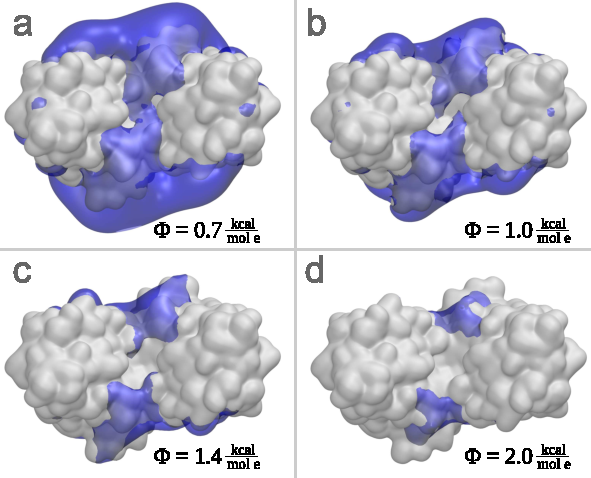
\includegraphics[width=1.0\textwidth]{gfx/bspred/il10_top_coulomb_isosurfaces_different_values_03_ds.pdf}
\caption[]{
Isosurface representation of IL-10's Coulomb potential (blue), shown for
multiple isovalues isovalues $\Phi$. The molecular surface of the IL-10 dimer is
shown in gray (structure taken from PDB ID 2ILK).
}
\label{fig:bspred:il10_multi_iso}
\end{figure}


\begin{figure}
\centering
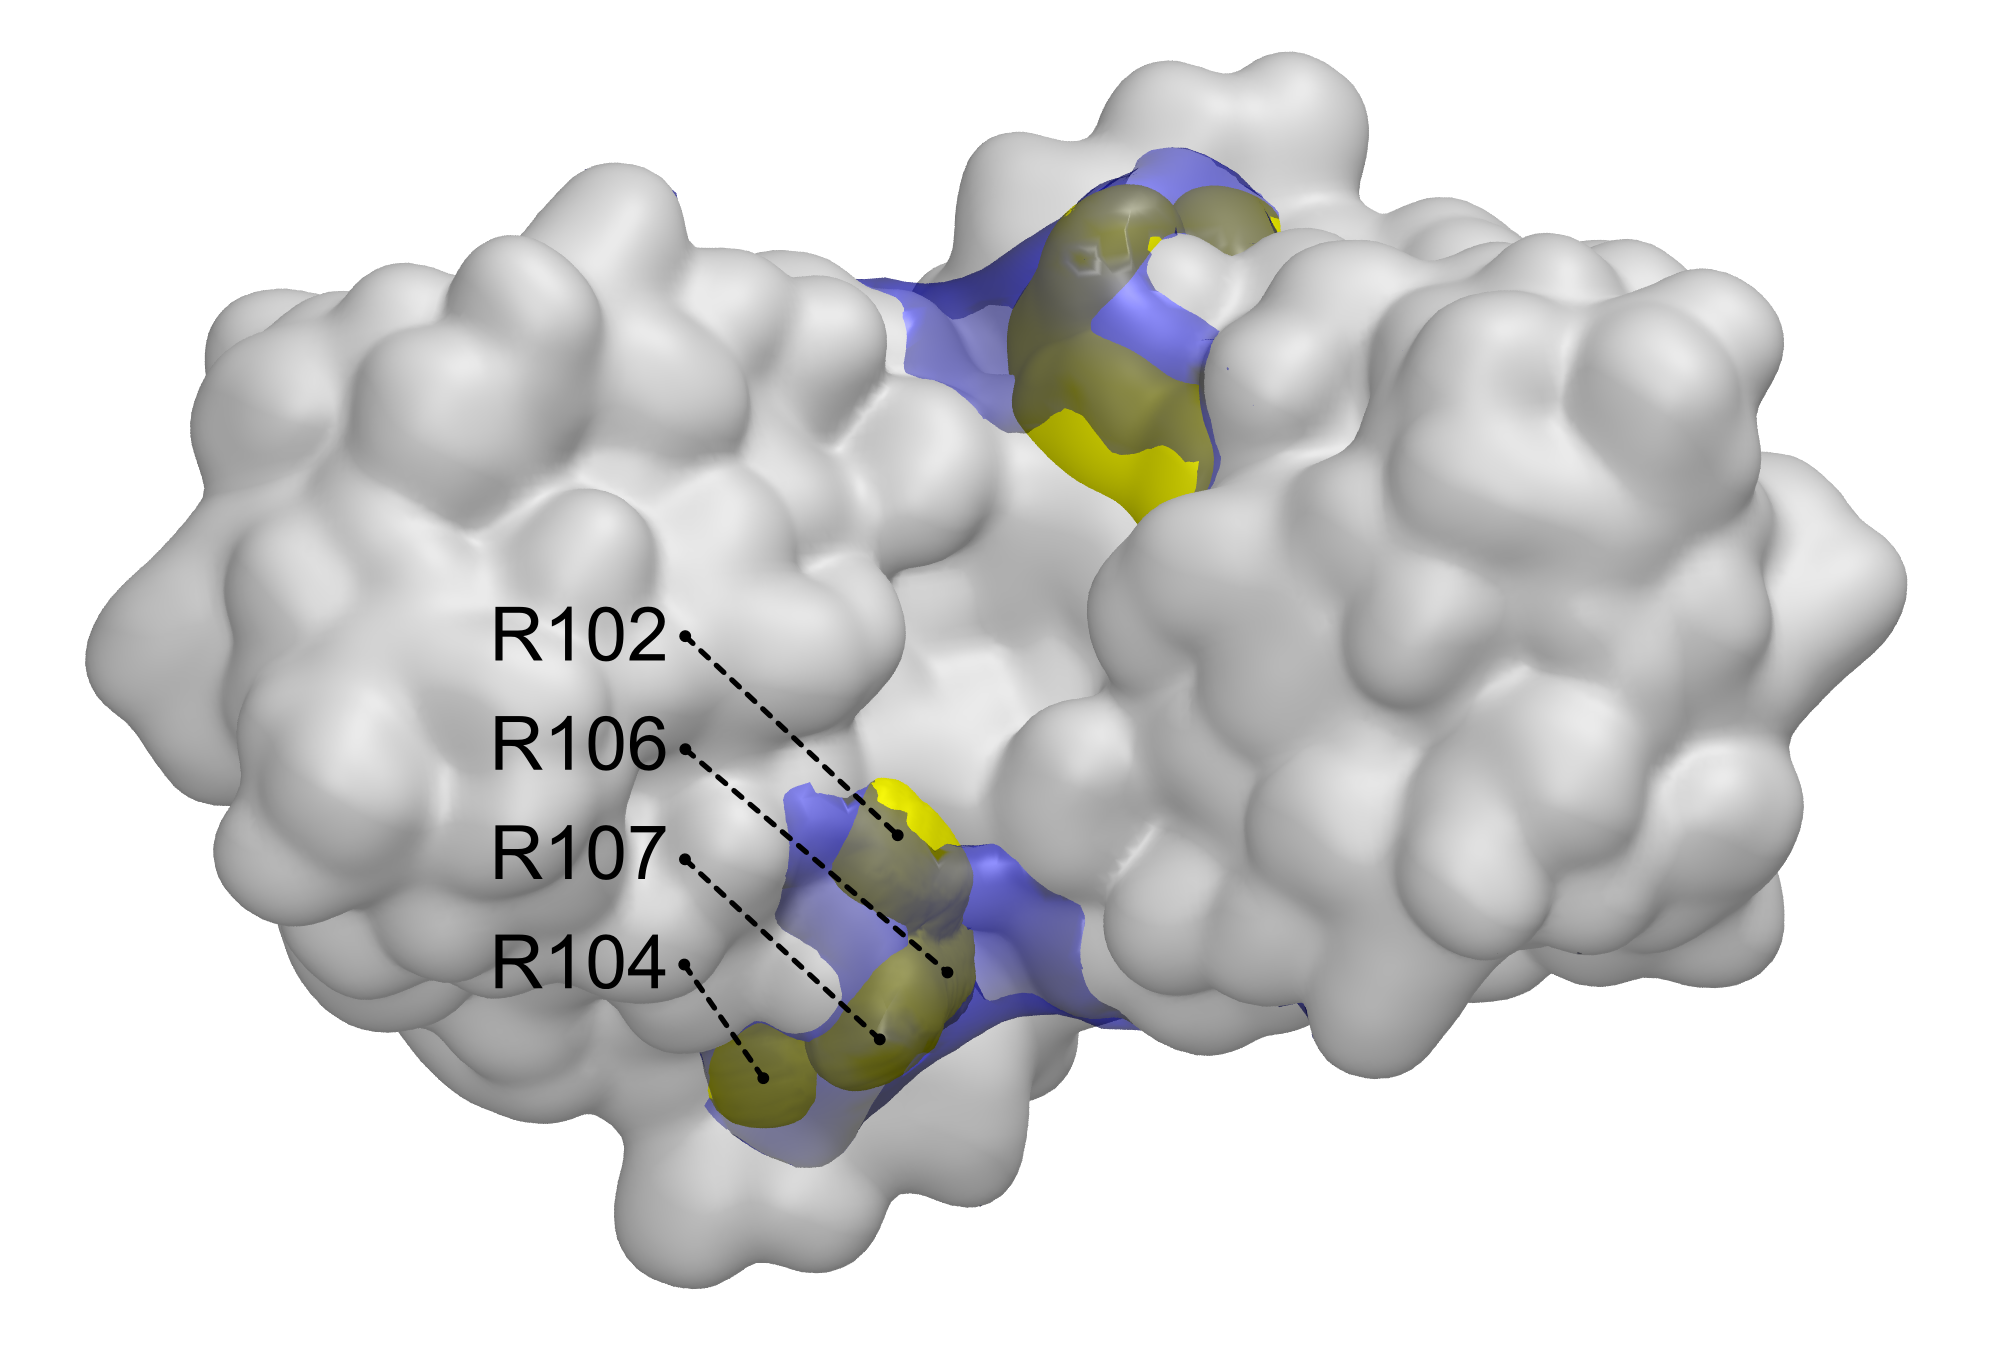
\includegraphics[width=0.9\textwidth]{gfx/bspred/SI_figure_IL-10_coulomb_isosurface_1_9kcalmol.png}
\caption[]{
Isosurface representation of IL-10's Coulomb potential with the isovalue $\Phi =
\SI{1.9}{\kilo\calory\per\mole\per\elementarycharge}$ (blue). The molecular
surface of the IL-10 dimer is shown in gray, the molecular surface of arginines
102, 104, 106, 107 is shown in yellow (structure taken from PDB ID 2ILK). This
representation allows to see where the Coulomb potential (for a given isovalue)
protrudes into space further than the molecular surface, and has been shown to
provide useful evidence about where GAGs bind to a protein \hl{(REF)}. Hence,
IL-10-GAG interaction most likely takes place within the two symmetrically
arranged regions indicated here.
}
\label{fig:bspred:il10_estatic_pred}
\end{figure}


\subsubsection{Electrostatic potential analysis in protein-GAG systems}

\hl{Generalize this section, keep details for DMD chapter. At the moment most of
this is simply copied from the DMD manuscript.}

The electrostatic potential often dominates protein-GAG interaction
\cite{gandhi_structure_2008}. In this section, we discuss the electrostatic
properties of the receptors in the TDS with the goal to determine how these
properties could assist defining a receptor target region for DMD and also to be
able to relate docking performance to electrostatic characteristics of the
receptor.


\begin{figure}
\centering
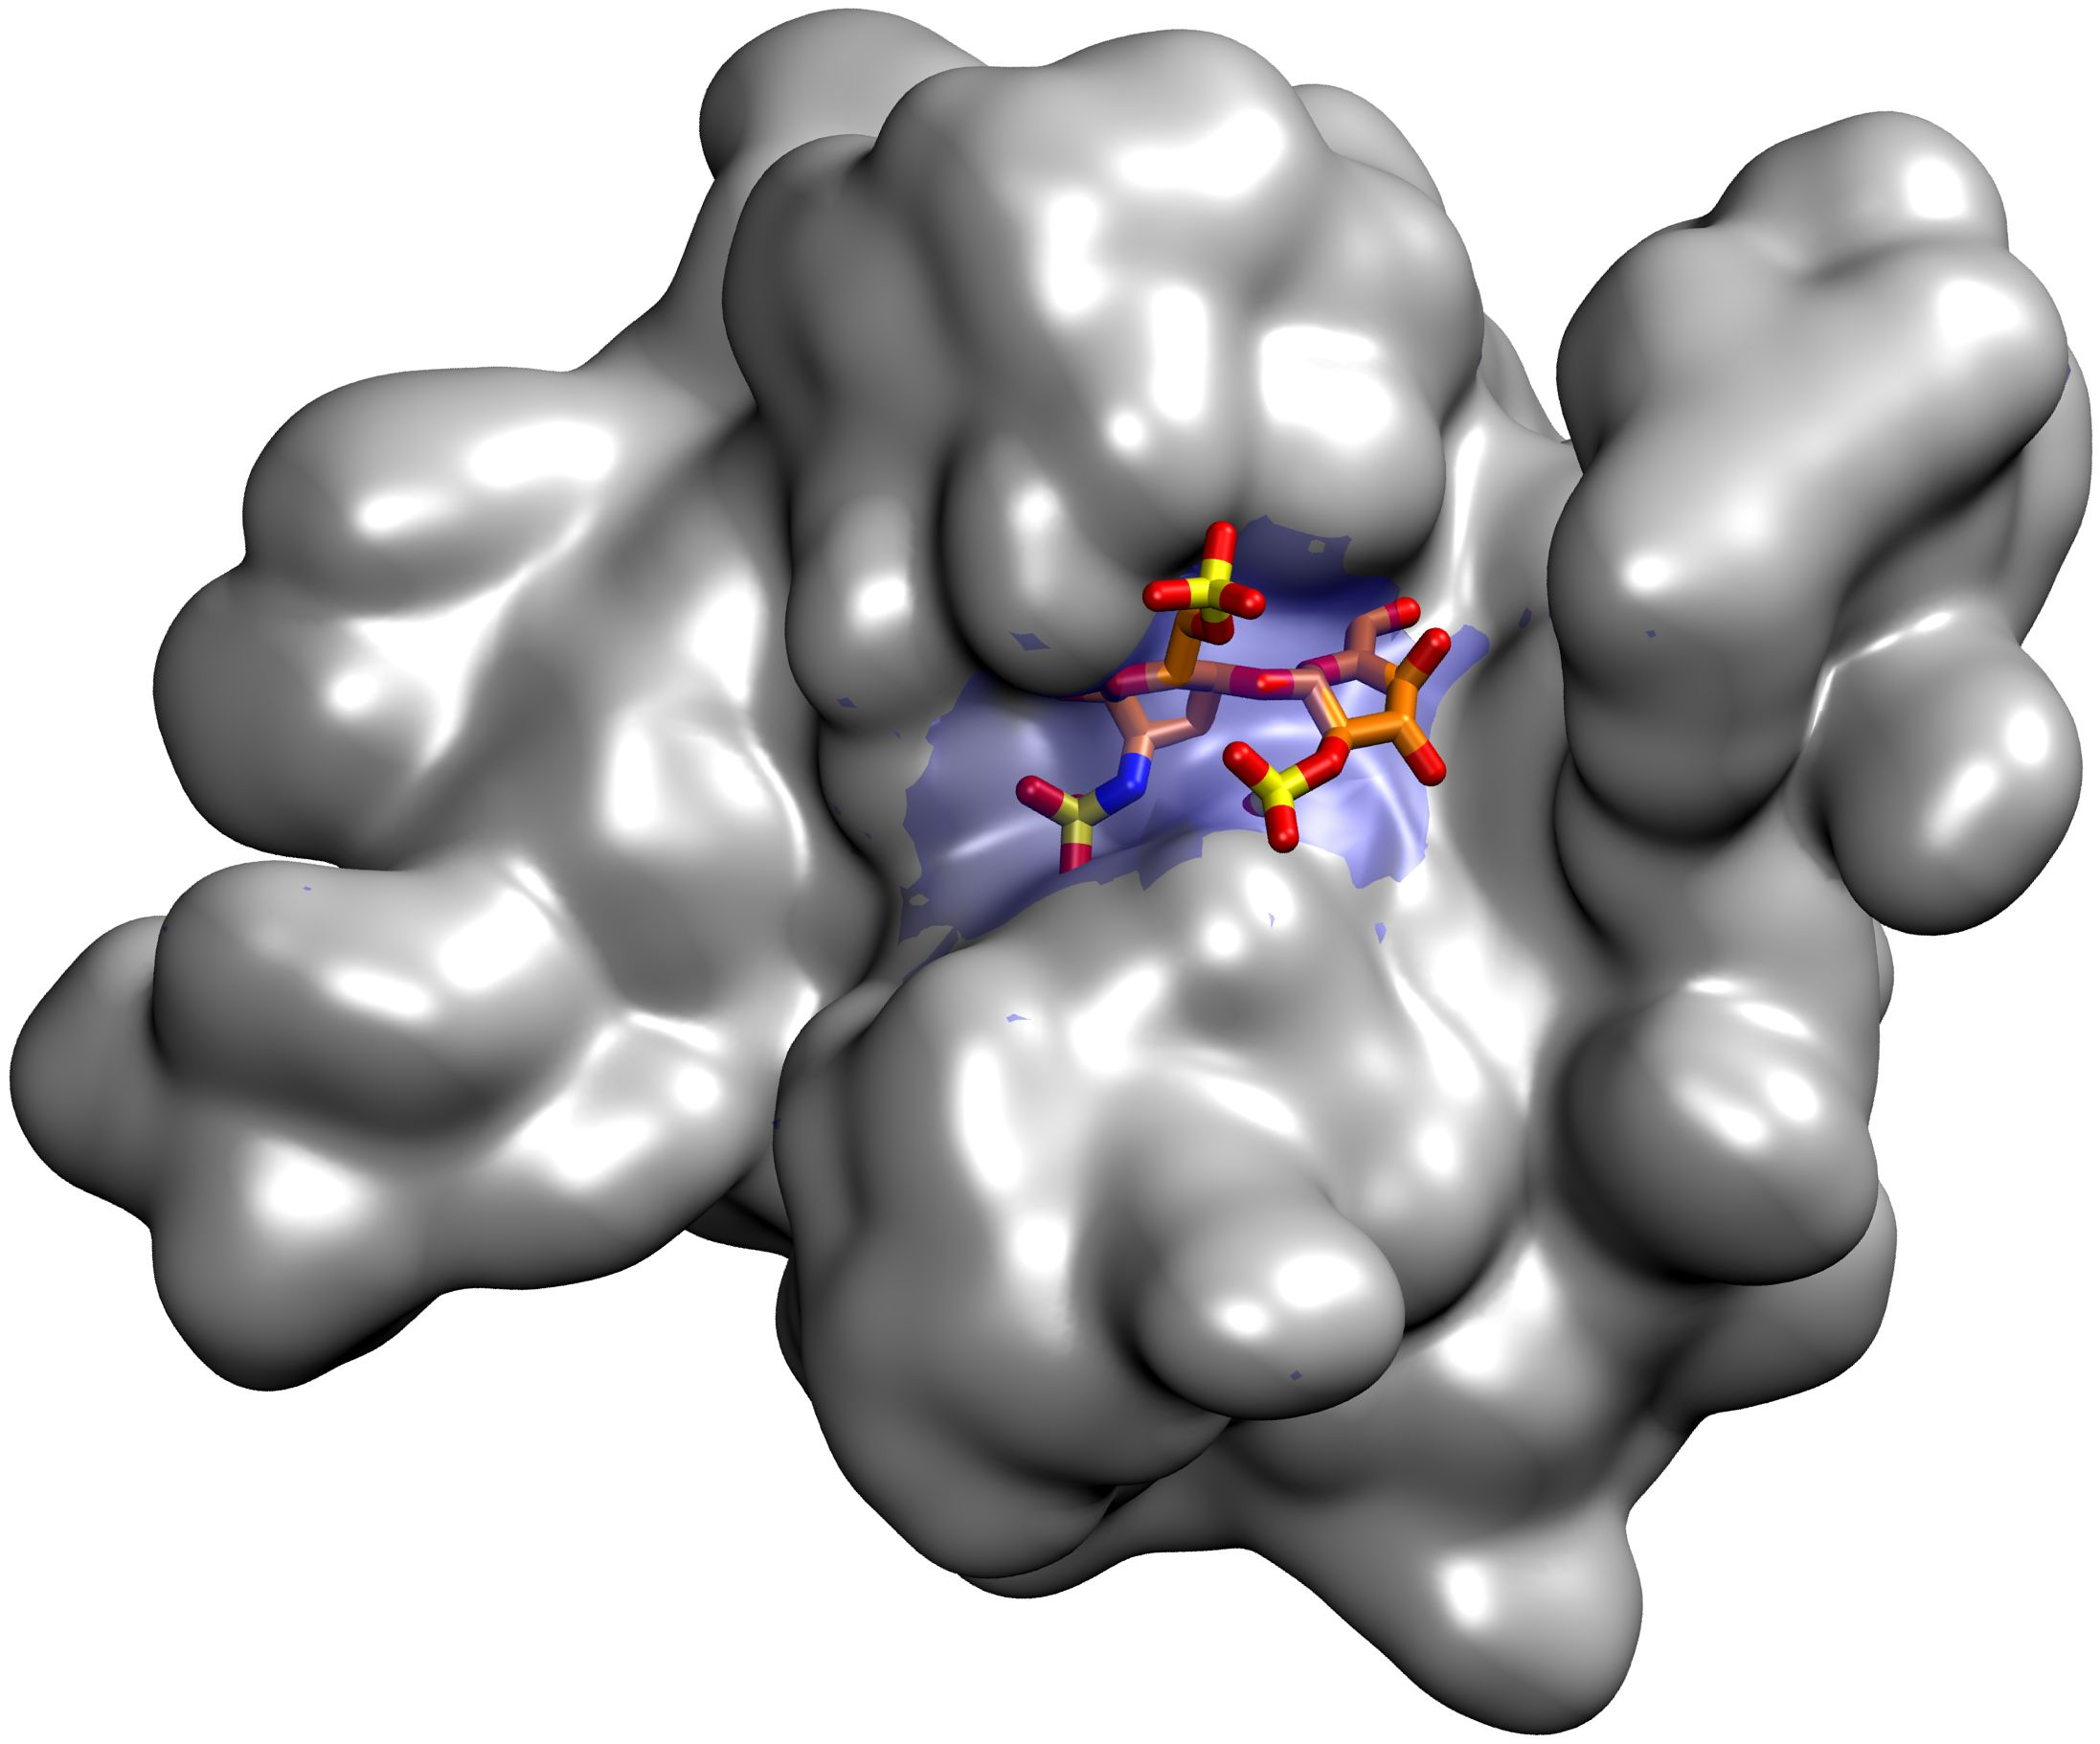
\includegraphics[width=0.9\textwidth]{gfx/bspred/sdf1_isopot_8_5_view1_rotated_jcc_pub_001.jpg}
\caption[]{
Isosurface representation of SDF-1's electrostatic potential with the isovalue
$\Phi = 8.5\,\mathrm{kcal\,mol^{-1}\,e^{-1}}$ (blue). The molecular surface of
the SDF-1 dimer is shown in grey, the heparin ligand as determined
experimentally (PDB ID 2NWG) is shown as sticks with C atoms in orange.
}
\label{fig:bspred:sdf1_estatic}
\end{figure}

 For
CD44-HA, the net electrostatic interaction between both molecules is slightly
repulsive. There is no obvious relation between the electrostatic properties of
the receptor and the binding site location. CathK and CathKmut exhibit
electrostatic attraction for negatively charged molecules in the experimentally
observed ligand binding site as well as in an adjacent region. We observe that
electrostatic potential analysis provides a clear idea whether GAG-binding to a
given receptor is mainly driven by Coulomb interaction. If a protein is known to
bind GAGs, and the electrostatic potential topology is as unambiguous as in case
of SDF-1 or FGF2, a GAG binding site prediction based on the presented procedure
is reliable. Visualization of the electrostatic potential can also be helpful to
\textit{a priori} exclude regions of the receptor surface when repulsive to
negatively charged ligands. Furthermore, this analysis shows that knowledge
about the electrostatic potential distribution in space can be used to choose a
reasonable ligand \enquote{entry lane} orientation for the tMD pulling process.


\begin{figure}
\centering
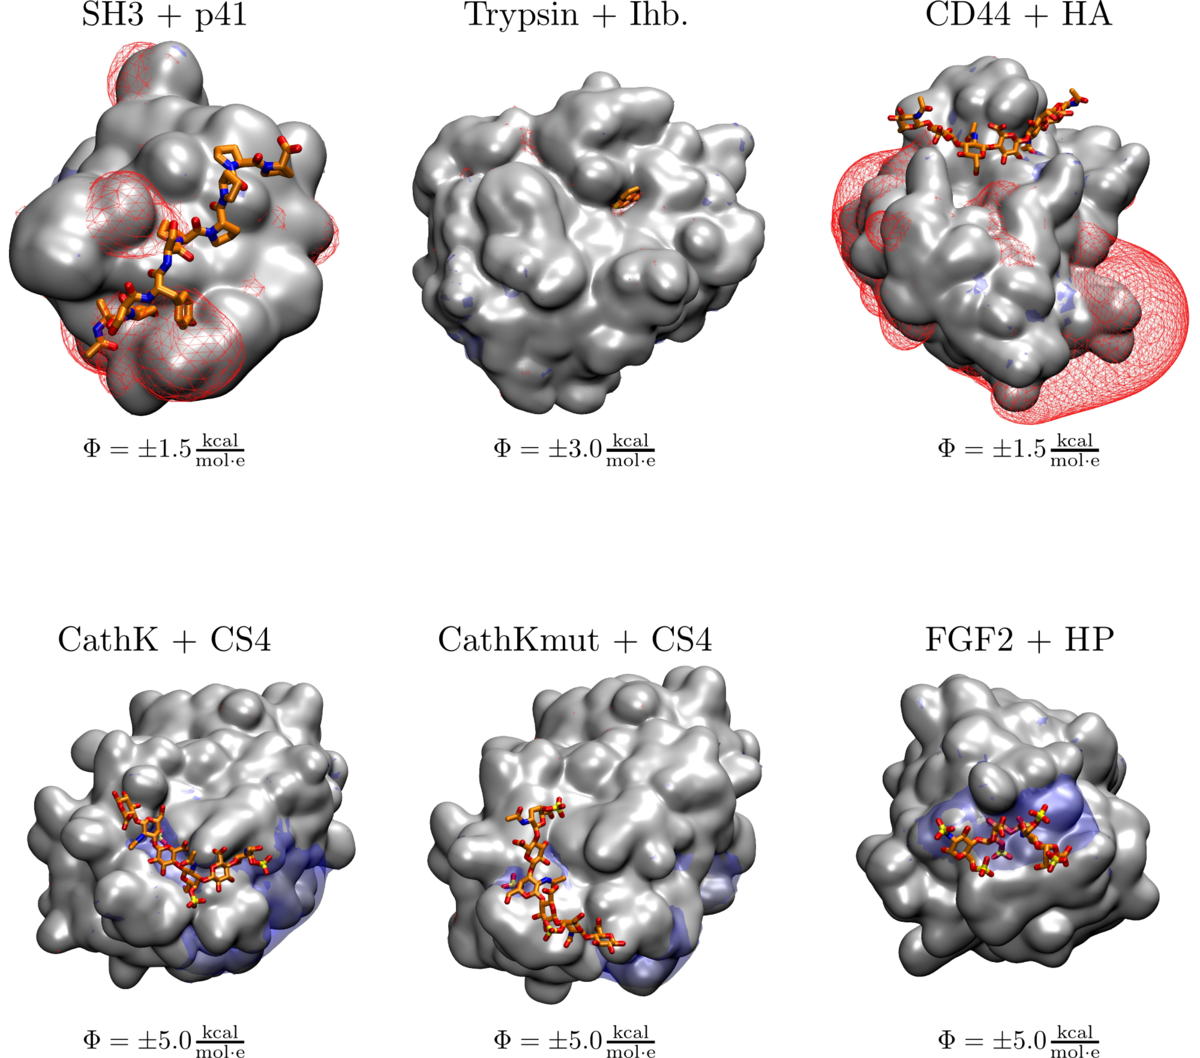
\includegraphics[width=0.9\textwidth]{gfx/bspred/suppl_figure_estatic_distributions_004_1200.png}
\caption[]{
Visualization of the electrostatic potential of the receptors from the TDS
(molecular surfaces in gray) with their ligands as experimentally determined
(shown as sticks with C atoms in orange). Blue/red: Isosurface representation of
the receptor's electrostatic potential with isovalue Ф (attractive/repulsive for
negatively charged molecules, respectively).
}
\label{fig:bspred:various_estatic}
\end{figure}


\hl{Create more convincing Figure than bspred:variousestatic.
Include more interesting complexes, remove uninteresting ones.}

The SH3-p41 complex is dominated by non-polar interactions, rendering the
Coulomb potential analysis inconclusive. Recognition of the Trypsin inhibitor in
its  binding pocket is affected by polar interactions. The electrostatic
potential, however, does not display clear characteristics to predict a binding
region.








\hl{INCORPORATE:} The method surely is more useful than the popular method of
heparin binding site consensus sequence search (cardin, weintraub) (hileman,
linhardt), which has already been applied to interleukin-10 before. Its about
structure, not sequence, that is also why Forster and Mulloy state that
\enquote{though some 'consensus sequences' for heparin binding have been
identified, they are neither necessary nor sufficient to define a heparin
binding site} \cite{hp_binding_sites_mulloy_2006}.
